%%%%%%%%%%%%%%%%%%%%%%%%%%%%%%%%%%%%%%%%%%%%%%%%% 
\chapter{Resultados} \label{sec_resultados}
%%%%%%,
%%%%%%%%%%%%%%%%%%%%%%%%%%%%%%%%%%%%%%%%%%% 

% caracteristicas dos pacientes diagnosticados com COVID-19
\section{Participantes}

\blue{O perfil dos participantes é apresentado na Tabela \ref{tab_dados_perfil}. Do conjunto de dados utilizado no estudo, 565.649 (96,82\%) casos possuem evolução conhecida como recuperação, e 18.579 (3,18\%) são casos que tiveram óbito comprovado por COVID-19, onde a taxa de letalidade geral é de 3,07\% (n=18.579). Dos casos confirmados, pouco mais da metade é do sexo feminino (53,10\%, n=310.263), tendo o sexo masculino a maior taxa de letalidade proporcional (3,6\%, n=9.889). Entre as faixa-etárias, a maior concentração está entre 30 e 39 anos (20,86\%), sendo a faixa superior aos 70 anos a mais letal (43.74\%, n=7.909). Dentre os sintomas, destacamos a falta de ar/dispnéia como o sintoma com a maior taxa de letalidade (17,49\%, n=15.676). Em contra-ponto, a dor-de-garganta é o sintoma apresentado que possui a menor taxa de letalidade (1,39\%, n=2.952). }

% Please add the following required packages to your document preamble:
% \usepackage{multirow}
% \usepackage{longtable}
% Note: It may be necessary to compile the document several times to get a multi-page table to line up properly
\begin{longtable}{lllll}
\caption{Dados dos participantes}
\label{tab_dados_perfil}\\ \hline
Nome do atributo                                              &               & Infectados  & Óbitos & Proporção (\%) \\ \hline
\endfirsthead
%
\endhead
%
\multirow{2}{*}{SEXO}                                          & Masculino     & 273.965 & 9889         & 3,60           \\
                                                               & Feminino      & 310.263 & 8.690         & 2,80           \\ \hline
\multirow{12}{*}{FAIXA\_ETARIA}                                 & \textless{}1  & 4.133   & 4            & 0,09           \\
                                                               & 01 a 04       & 7.403   & 4            & 0,05           \\
                                                               & 05 a 09       & 9.267   & 2            & 0,02           \\
                                                               & 10 a 14       & 13390  & 5            & 0,03           \\
                                                               & 15 a 19       & 30.292  & 19           & 0,06           \\
                                                               & 20 a 29       & 108.501 & 225           & 0,20           \\
                                                               & 30 a 39       & 121.926 & 758          & 0,62           \\
                                                               & 40 a 49       & 104.102 & 1.716          & 1,64           \\
                                                               & 50 a 59       & 88.424  & 3.138         & 3,54           \\
                                                               & 60 a 69       & 57.058  & 4.799         & 8,41           \\
                                                               & 70 a 79       & 27.233  &   4.516       & 16,58          \\
                                                               & 80 e mais     & 12.490  & 3.393         & 27,16          \\ \hline
FEBRE                                                          & Sim  & 198.357 & 8.909  & 4,49 \\
                                                               & Não           & 385.871 & 9.670         & 2,50           \\ \hline
TOSSE                                                          & Sim   & 270.337 & 10.873         & 4,02           \\
                                                               & Não           & 313.891 & 7.706         & 2,45           \\ \hline
GARGANTA                                                       & Sim  & 211.297 &  2.952  & 1,39           \\
                                                               & Não & 372.931 & 2.952        & 4,19           \\ \hline
DISPNEIA                                                       & Sim           & 89.606 & 15.676        & 17,49          \\
                                                               & Não           & 494.622 & 2.903         & 0,58           \\ \hline
GESTANTE                                                       & Sim           & 3.157   & 47           & 1,48           \\
                                                               & Não           & 581.071 & 18.532        & 3,18           \\ \hline
                                                               
SRAG                                                       & Sim           & 51.691   & 18.579           & 35,94           \\
                                                               & Não           & 532.537 & 0        & 0,0           \\ \hline
CARDIOPATIA                                                    & Sim           & 16.981  & 7.728         & 45,50          \\
                                                               & Não           & 556.396 & 10.851         & 1,91          \\ \hline
DIABETES                                                       & Sim           & 22.627  & 5.593         & 24,71          \\
                                                               & Não           & 561.601 & 17.034         & 2,31           \\ \hline
DOENCA\_RESPIRATORIA                                           & Sim           & 3.566   & 1.552         & 43,52          \\
                                                               & Não           & 563.635 & 17.027        & 2,93           \\ \hline
PROBLEMA\_RENAL                                                & Sim           & 2254   & 861         & 38,19          \\
                                                               & Não           & 581.974 & 17.718        & 3,04          \\ \hline
OBESIDADE                                                      & Sim           & 10.855   & 2.868         & 26,42          \\
                                                               & Não           & 573.373 & 15.711        & 2,74           \\ \hline
DOENCA\_CROMOSSOMICA                                           & Sim           & 141    & 83           & 41,13          \\
                                                               & Não           & 584.087 & 18.521        & 3,17           \\ \hline
\end{longtable}


\section{Desenvolvimento do modelo}
\red{Aplicamos o algoritmo de Floresta aleatória, utilizando 100 árvores de decisão (\texttt{n\_estimators}) no processo e com 4 de profundidade máxima (\texttt{max\_depth}), pois foram os melhores hiperparâmetros retornados pela busca em grade com validação cruzada (k = 5). Como o conjunto de dados de teste é desbalanceado, possuindo 395.954 (96,82\%) casos recuperados e 13.005 (3,18\%) óbitos, optamos por utilizar da técnica de subamostragem aleatória (\textit{random under sampling}) \cite{anand2010approach} nos dados de treino. }

\blue{O coeficiente de correlação de Pearson entre as variáveis independentes pode ser observado na Figura \ref{figura_corr}. Podemos constatar uma variação de -0,8 a 0,6, e que as variáveis que possuem uma maior dependência (>= 0.2) com a variável resposta (EVOLUCAO) são SRAG, DISPNEIA, CARDIOPATIA, DIABETES, DOENCA\_RESPIRATORIA e OBESIDADE (\textit{i.e.}, variáveis que possuem maior correlação). E de acordo com grau de impureza de Gini, constatamos a influência relativa das \textit{top} 5 características na classificação predita pelo modelo, a saber: SRAG, FAIXAETARIA, CARDIOPATIA, DISPNEIA e DIABETES (Figura \ref{figura_feature_importance}).}

\begin{figure}[H]
\caption{Matriz de correlação de Pearson}
\centering % para centralizarmos a figura
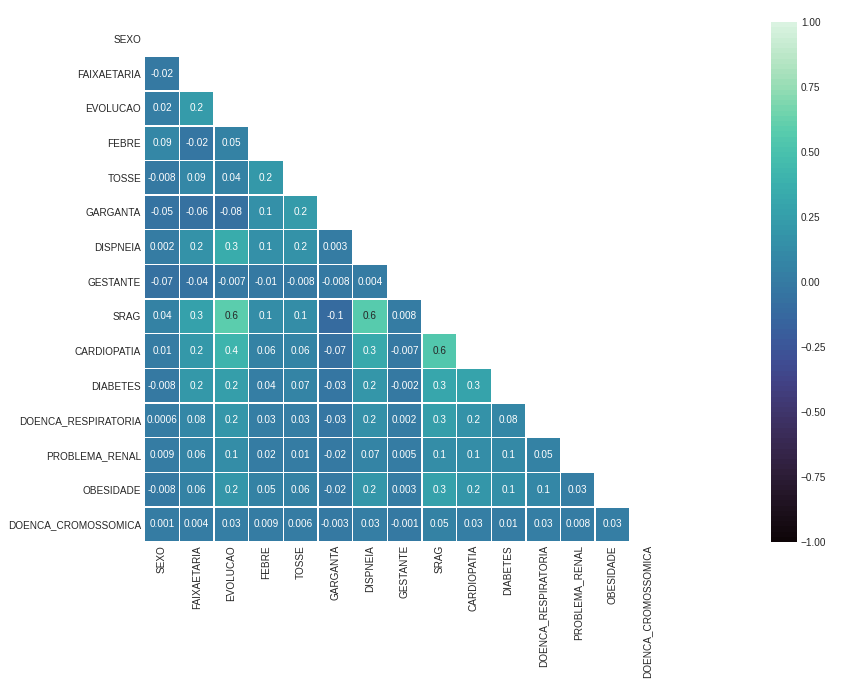
\includegraphics[width=\textwidth]{figuras/corr.png}
\label{figura_corr}
\end{figure}
\begin{figure}[H]
\caption{Índice de impureza de Gini}
\centering % para centralizarmos a figura
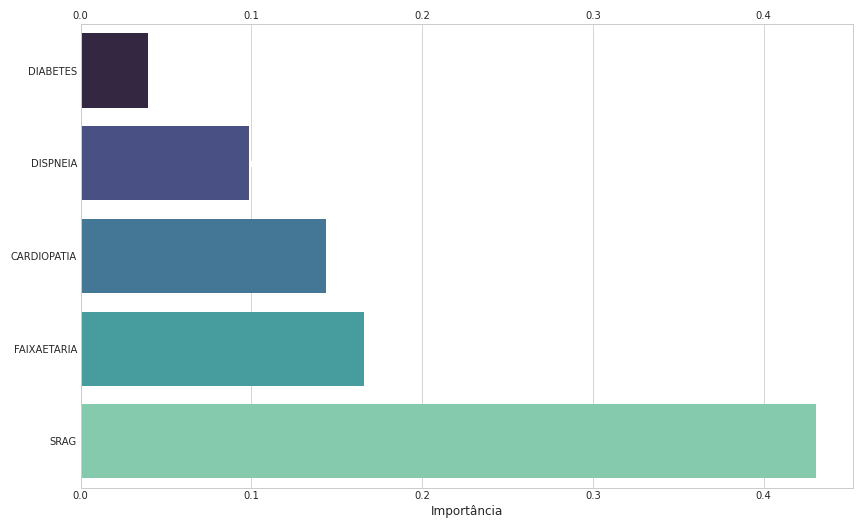
\includegraphics[width=14cm]{figuras/feature_importance.png}
\label{figura_feature_importance}
\end{figure}

\red{O fluxo geral para o uso do modelo proposto pode ser visualizado na Figura \ref{figura_geral}. Primeiramente, os dados clínicos e sintomas do paciente são coletados (A) e inseridos no modelo já treinado (B). Com o desfecho predito pelo modelo (C), o profissional da saúde em atividade (D) pode basear-se para tomar a decisão se aquele indivíduo pode ou não ocupar a vaga de leito de UTI (E).}

\begin{figure}[H]
\caption{Fluxo de uso do modelo}
\centering % para centralizarmos a figura

\includegraphics[width=\textwidth]{figuras/fluxo_geral.png}
\label{figura_geral}
\end{figure}

\section{Avaliação e Validação do modelo}

O conjunto inicial dos dados possuía 584.228 registros e um total de 18.579 óbitos. O conjunto de treino e teste possui 408.959 registros, sendo 3,18\% (n=13.005) óbitos. O conjunto de validação possui a mesma distribuição, sendo 5.574 óbitos. A Figura \ref{figura_train_test} ilustra a divisão dos dados em cada etapa de treino, teste e validação. Os valores das pontuações médias após a validação cruzada (5-V.C.) do modelo de floresta aleatória, juntamente com seus intervalos de confiança com nível de confiança de 95\% (I.C. = 95\%) podem ser vistos na Tabela \ref{tab_performance}. O modelo com menos registros de óbito (com raça/cor) possui o pior desempenho e foi descartado das melhorias posteriores (subamostragem e ajuste de hiperparâmetros).

\begin{figure}[H]
\caption{Fluxo dos dados de treino, teste e validação}
\centering % para centralizarmos a figura
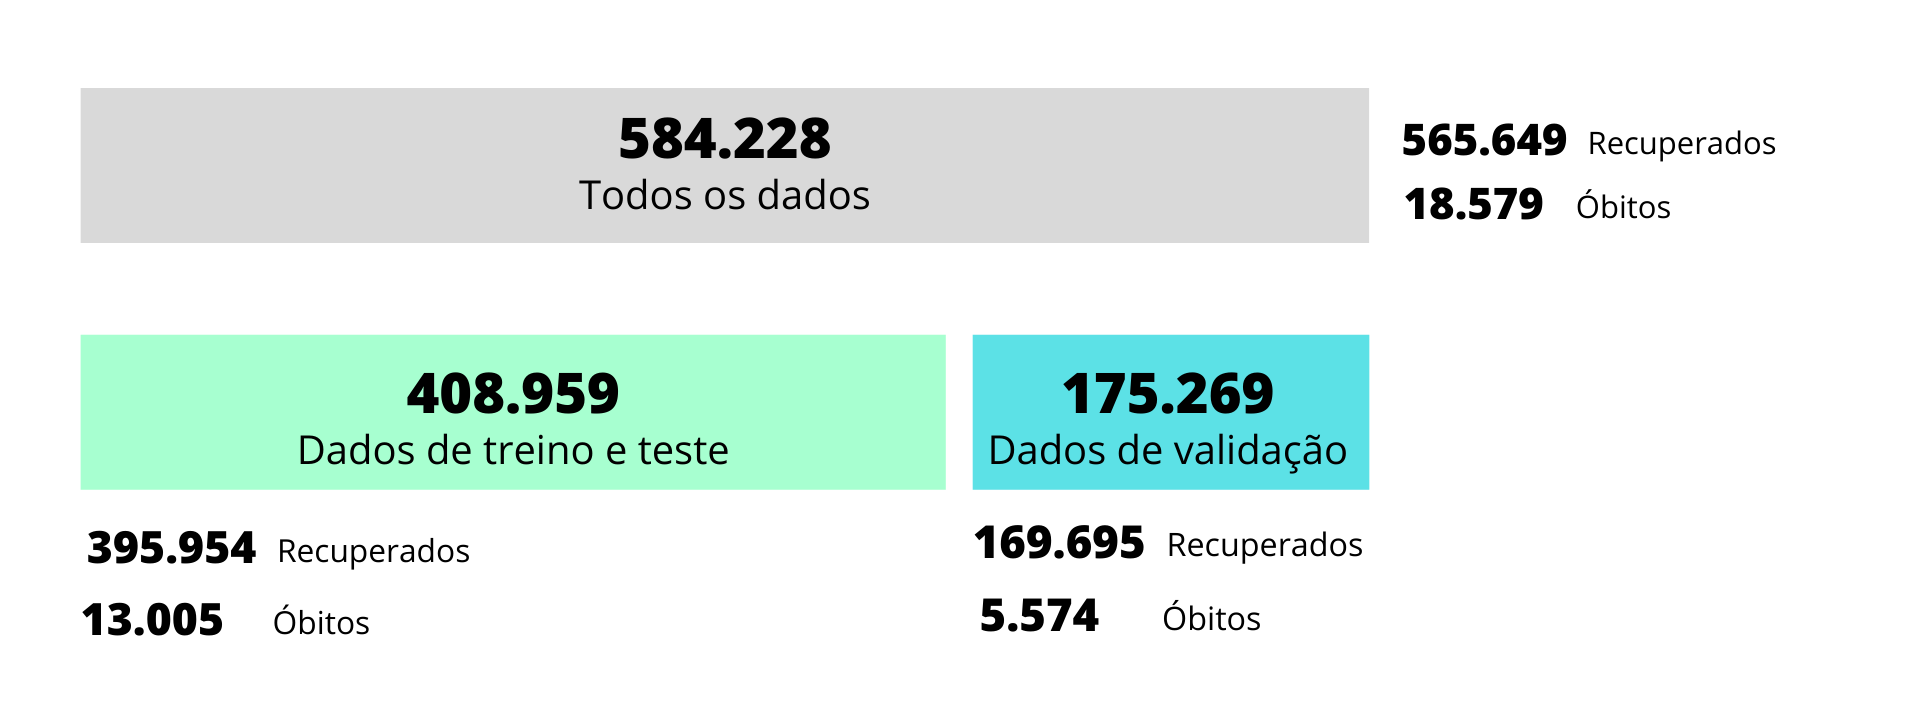
\includegraphics[width=\textwidth]{figuras/fluxo_treino_teste.png}
\label{figura_train_test}
\end{figure}

\begin{table}[H]
\centering
\caption{Performance do modelo}
\label{tab_performance}
\begin{tabular}{l|l|l}
\multicolumn{1}{l}{}                                                                                                   & \multicolumn{2}{l}{Pontuação AUC-ROC}  \\ 
\cline{2-3}
\multicolumn{1}{l}{}                                                                                                   & Média (5-V.C.) & I.C. = 95 \%           \\ 
\hline
\begin{tabular}[c]{@{}l@{}}Floresta aleatória \\(com raça/cor)\end{tabular}                                            & 0,539         & (0,528 - 0,550)         \\ 
\hline
\begin{tabular}[c]{@{}l@{}}Floresta aleatória \\(linha de base)~\end{tabular}                                          & 0,705         & (0,694 - 0,716)        \\ 
\hline
\begin{tabular}[c]{@{}l@{}}Floresta aleatória\\(subamostragem aleatória)\end{tabular}                                  & 0,969         & (0,968 - 0,970)        \\ 
\hline
\begin{tabular}[c]{@{}l@{}}Floresta aleatória\\(subamostragem aleatória +\\ajuste de hiperparâmetro)\end{tabular} & 0,981         & (0,981 - 0,982)        \\
\hline
\end{tabular}
\end{table}

\blue{Utilizamos uma matriz de confusão (Figura \ref{figura_confusion_matrix}) para descrever e visualizar a performance do classificador nos dados de validação e também para prover \textit{insights} sobre onde o modelo errou. É importante salientar que pontuação AUC-ROC é derivada desta matriz, que informa os falsos positivos e negativos, bem como os classificados corretamente. No nosso contexto, a nossa classe positiva são os casos de óbitos e a classe negativa são os casos recuperados. Podemos observar na matriz que apenas 5,92\% (n=10.045) casos recuperados foram classificados errôneamente (falsos positivos) e que todos os casos de óbito foram classificados corretamente (\textit{i.e.}, sem falsos negativos). Como o modelo performou acima de 0,90 de pontuação AUC-ROC, podemos classificá-lo como excelente discriminador \cite{hosmer2013applied}.}

\begin{figure}[H]
\caption{Matriz de confusão conjunto de validação}
\centering % para centralizarmos a figura
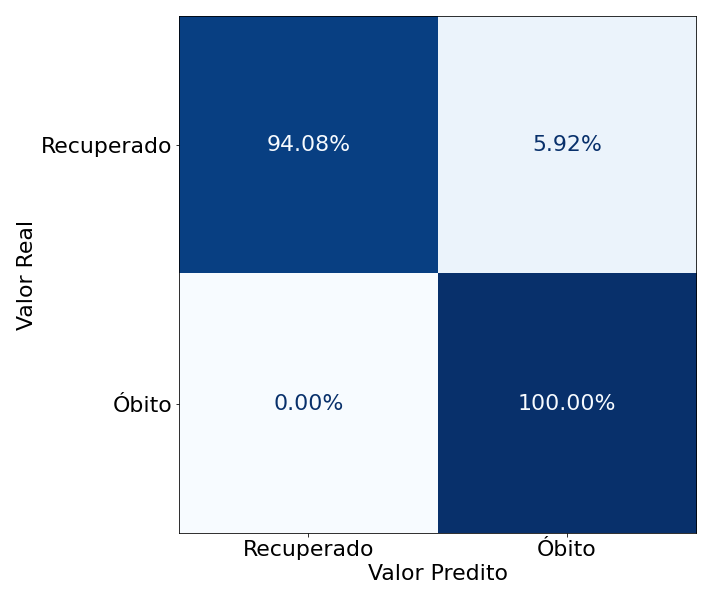
\includegraphics[width=12cm]{figuras/confusion_matrix.png}
\label{figura_confusion_matrix}
\end{figure}



%\section{Interpretabilidade}

%Na real eu n sei bem o que vai ficar aqui.